% -*- coding: utf-8 -*-
\section{Dos estilos de cálculo: sintético frente a analítico}

A lo largo del curso hemos utilizado la deducción natural (temas~\ref{cap:dn-prop} y~\ref{cap:dn-lpo}) como cálculo de demostración. Sin embargo, en la historia de la lógica existen dos familias de cálculos:

\begin{enumerate}
    \item \textbf{Cálculos sintéticos (o generativos).}  
    Tanto los sistemas axiomáticos al estilo de Frege y Hilbert como
    la deducción natural de Gentzen son cálculos sintéticos. Parten de
    axiomas o de premisas iniciales y proceden hacia
      adelante, generando fórmulas paso a paso 
    mediante reglas de inferencia. La deducción natural modela
    el proceso de demostración directa: «tengo estas
    premisas, aplico una secuencia de reglas y llego a la conclusión». 
    
    \item \textbf{Cálculos analíticos (o de descomposición).}  
    Desarrollados por Evert Beth (1955), Jaakko Hintikka (1955) y
    Raymond Smullyan (1968), los \textbf{tableaux semánticos} proceden
    en sentido inverso: parten de las fórmulas complejas que queremos
    examinar y las descomponen en sus partes
      constitutivas. Su estrategia no es «construir una prueba» paso
    a paso, sino buscar sistemáticamente una estructura
      semántica o modelo que haga verdadero un conjunto de fórmulas;
    si la búsqueda fracasa en todas las ramas, ese fracaso es la
    prueba. También suele contarse entre los cálculos analíticos el de resolución, propuesto
    por John Alan Robinson (1965): como los tableaux, trabaja por
    refutación y es la base de muchos demostradores automáticos y del
    lenguaje de programación lógica Prolog.
\end{enumerate}

Mientras que la deducción natural responde a la pregunta sintética \emph{«¿Cómo justifico este enunciado paso a paso?»}, el cálculo de tableaux responde a la pregunta analítica \emph{«¿Es posible concebir una situación o mundo donde estas premisas sean verdaderas y la conclusión falsa?»}.

Esta diferencia tiene consecuencias prácticas. En deducción natural hay que decidir qué hipótesis abrir, qué fórmulas intermedias buscar o cuándo recurrir a la reducción al absurdo, y nada garantiza que una elección sea la buena. En un tableau no hay que inventar nada: las reglas solo descomponen las fórmulas que ya están en la rama, de modo que su aplicación puede mecanizarse por completo. En lógica proposicional el proceso siempre termina y proporciona un procedimiento de decisión; en primer orden, una aplicación sistemática de las reglas encuentra un tableau cerrado siempre que lo haya, aunque puede no terminar cuando no lo hay (sección~\ref{sec:ramas-infinitas}). Por eso los tableaux están también en la base de muchos demostradores automáticos, que usan variables libres y unificación para no tener que probar a ciegas una constante tras otra en la regla $\gamma$ (Fitting, 1996), y de los razonadores para lógicas modales y para las lógicas de descripción con las que se construyen ontologías. No son, sin embargo, el método más eficiente en todos los casos: hay fórmulas proposicionales cuyos tableaux cerrados son mucho más largos que su tabla de verdad (D'Agostino, 1992).

En este tema trabajamos con lenguajes sin el símbolo de identidad ni símbolos de función. Si el tableau encuentra un contramodelo (una rama abierta y completa), el argumento queda refutado; si el tableau descarta todas las posibilidades por contradicción (todas las ramas se cierran), queda demostrado que la conclusión se sigue de las premisas.

\section{Clasificación uniforme de fórmulas (Raymond Smullyan)}

Un tableau es un árbol. En su raíz se escriben las fórmulas de
partida (para comprobar si $\Gamma \models A$, las de $\Gamma$ y
$\neg A$), que luego se descomponen en otras más simples. Si una
fórmula exige que otras dos sean verdaderas, ambas se añaden a la
misma rama; si basta con que lo sea una de ellas, la rama se bifurca en
dos, una para cada posibilidad. Cada rama describe una situación
posible; si contiene una fórmula y su negación, la situación es
imposible y la rama se cierra (sección~\ref{sec:reglas-tableau}).

Para evitar tener que formular decenas de reglas \emph{ad hoc} para cada combinación de conectivas y negaciones, el lógico estadounidense Raymond Smullyan introdujo una clasificación uniforme en cuatro categorías:

\subsection{Fórmulas proposicionales: tipos \texorpdfstring{$\alpha$}{alpha} y \texorpdfstring{$\beta$}{beta}}

\begin{itemize}
    \item \textbf{Fórmulas de tipo $\alpha$ (conjuntivas, no ramifican).}  
    Son fórmulas que son verdaderas si y solo si lo son sus dos componentes. Se descomponen linealmente en la misma rama:
    \begin{center}
    \begin{tabular}{|c|c|c|}
    \hline
    $\alpha$ & $\alpha_1$ & $\alpha_2$ \\
    \hline
    $A \land B$ & $A$ & $B$ \\
    $\neg (A \lor B)$ & $\neg A$ & $\neg B$ \\
    $\neg (A \to B)$ & $A$ & $\neg B$ \\
    \hline
    \end{tabular}
    \end{center}
    
    \item \textbf{Fórmulas de tipo $\beta$ (disyuntivas, ramifican).}  
    Son fórmulas que son verdaderas si y solo si lo es al menos uno de sus componentes. Exigen bifurcar el árbol en dos ramas alternativas:
    \begin{center}
    \begin{tabular}{|c|c|c|}
    \hline
    $\beta$ & $\beta_1$ & $\beta_2$ \\
    \hline
    $A \lor B$ & $A$ & $B$ \\
    $\neg (A \land B)$ & $\neg A$ & $\neg B$ \\
    $A \to B$ & $\neg A$ & $B$ \\
    $A \leftrightarrow B$ & $A \land B$ & $\neg A \land \neg B$ \\
    $\neg (A \leftrightarrow B)$ & $A \land \neg B$ & $\neg A \land B$ \\
    \hline
    \end{tabular}
    \end{center}
\end{itemize}

\subsection{Fórmulas cuantificadas: tipos \texorpdfstring{$\gamma$}{gamma} y \texorpdfstring{$\delta$}{delta}}

\begin{itemize}
    \item \textbf{Fórmulas de tipo $\gamma$ (universales).}  
    Equivalen a una afirmación universal ($\forall x A(x)$ o $\neg \exists x A(x) \equiv \forall x \neg A(x)$). Se pueden instanciar con cualquier constante $c$ que aparezca en la rama:
    \begin{center}
    \begin{tabular}{|c|c|}
    \hline
    $\gamma$ & $\gamma(c)$ \\
    \hline
    $\forall x A(x)$ & $A(c)$ \\
    $\neg \exists x A(x)$ & $\neg A(c)$ \\
    \hline
    \end{tabular}
    \end{center}
    
    \item \textbf{Fórmulas de tipo $\delta$ (existenciales).} Equivalen a una afirmación existencial, como $\exists x A(x)$ o bien $\neg \forall x A(x)$. Exigen introducir una \textbf{constante testigo fresca} $a$ que no haya aparecido previamente en la rama:
    \begin{center}
    \begin{tabular}{|c|c|}
    \hline
    $\delta$ & $\delta(a)$ (con $a$ nueva) \\
    \hline
    $\exists x A(x)$ & $A(a)$ \\
    $\neg \forall x A(x)$ & $\neg A(a)$ \\
    \hline
    \end{tabular}
    \end{center}
\end{itemize}

\subsection{Fórmulas literales y doble negación (\texorpdfstring{$\sigma$}{sigma})}
\begin{itemize}
    \item \textbf{Literales.} Fórmulas atómicas ($P(c_1, \dots, c_n)$)
      o sus negaciones ($\neg P(c_1, \dots, c_n)$). No se
      descomponen más; constituyen los nodos básicos de evaluación.
    \item \textbf{Regla $\sigma$ (doble negación).} De $\neg\neg A$ se añade $A$ a la rama. (Smullyan trata $\neg\neg A$ como una fórmula $\alpha$ con $\alpha_1 = \alpha_2 = A$; aquí la presentamos aparte por claridad).
\end{itemize}

\section{Reglas de construcción y cierre de un tableau}\label{sec:reglas-tableau}

El árbol, que se dibuja con la raíz arriba, se construye de acuerdo con las siguientes pautas:

\begin{enumerate}
    \item \textbf{Inicio.} Se colocan las fórmulas del conjunto de partida como nodos iniciales en una columna vertical (el tronco del árbol).
    \item \textbf{Expansión no ramificada ($\alpha$, $\sigma$ y $\delta$).} Se añade el resultado al final de todas las ramas abiertas que pasen por la fórmula.
    \item \textbf{Expansión ramificada ($\beta$).} Cada rama abierta que pasa por la fórmula se bifurca en dos, con $\beta_1$ en una y $\beta_2$ en la otra.
    \item \textbf{Instanciación universal ($\gamma$).} Se añade $\gamma(c)$ para cada constante $c$ ya existente en la rama; si en la rama no hay todavía ninguna constante, se introduce una nueva. Si posteriormente aparecen nuevas constantes, la fórmula $\gamma$ debe volver a utilizarse con ellas (las fórmulas $\gamma$ nunca se «agotan»).
    \item \textbf{Regla de cierre.} Una rama queda \textbf{cerrada} en cuanto contiene una contradicción explícita: una fórmula $A$ y su negación $\neg A$. Lo más frecuente es que se cierre con un literal y su negación ($P(a)$ y $\neg P(a)$), pero no hace falta descomponer más $A$ si ya aparecen $A$ y $\neg A$ en la rama. Se marca el final de la rama con el símbolo $\bigotimes$. Una rama cerrada deja de expandirse.
\end{enumerate}

\subsection{Estado final de un tableau}
\begin{itemize}
    \item \textbf{Tableau cerrado.} Todas las ramas del árbol terminan en contradicción ($\bigotimes$). No existe ningún camino coherente para hacer verdaderas las fórmulas. Demuestra que el conjunto de partida es insatisfacible.
    \item \textbf{Tableau abierto y completo.} Al menos una rama permanece sin contradicción y se han aplicado todas las reglas posibles sobre sus fórmulas. Demuestra que el conjunto de partida es satisfacible.
\end{itemize}

\subsection{Estrategia heurística: orden de expansión}

Para evitar un crecimiento innecesario del árbol, conviene seguir una heurística habitual de prioridad (no afecta a la corrección del método, solo a su eficiencia, siempre que ninguna fórmula quede sin expandir indefinidamente; Smullyan ya recomendaba aplicar las reglas $\alpha$ antes que las $\beta$):
\begin{center}
\textbf{Prioridad de expansión: } $\alpha$ (y $\sigma$) $\ \longrightarrow \ \delta \ \longrightarrow \ \gamma \ \longrightarrow \ \beta$
\end{center}
\begin{enumerate}
    \item \textbf{Prioridad 1 ($\alpha$ y $\sigma$).} Descomponer primero todas las fórmulas que no ramifican. 
    \item \textbf{Prioridad 2 ($\delta$).} Descomponer los existenciales introduciendo una constante fresca $a$.
    \item \textbf{Prioridad 3 ($\gamma$).} Instanciar los universales con las constantes ya generadas por las reglas $\delta$ o presentes previamente en la rama (y solo con una nueva si no hay ninguna).
    \item \textbf{Prioridad 4 ($\beta$).} Posponer las bifurcaciones disyuntivas hasta que no quede otra opción. Si ramificamos prematuramente, cualquier fórmula pendiente tendrá que descomponerse por duplicado en cada una de las nuevas ramas.
\end{enumerate}

\begin{ejemplo}[Tableau proposicional: silogismo disyuntivo]
Comprobamos la inferencia $(p \lor q) \land \neg p \models q$.
Colocamos la premisa y la negación de la conclusión en la raíz, dado
que estamos buscando un modo de hacer verdadera la premisa y falsa la
conclusión:
\begin{center}
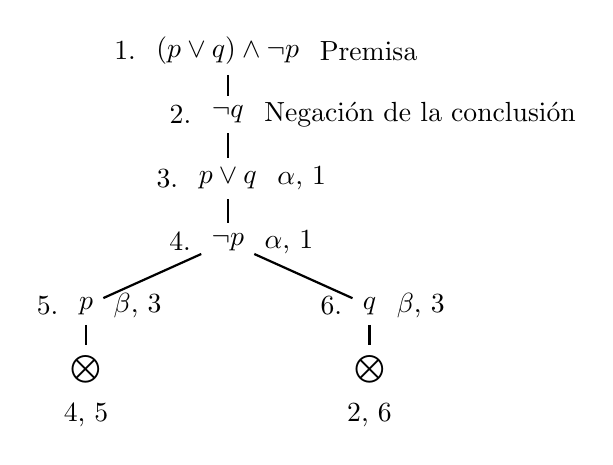
\begin{tikzpicture}[scale=0.9, -, thick, level/.style={sibling distance=4cm,level distance=.9cm}]
  \node[label=left:{1.},label=right:{Premisa}] (r1) {$(p \lor q) \land \neg p$}
  child {
    node[label=left:{2.},label=right:{Negación de la conclusión}] {$\neg q$}
    child {
      node[label=left:{3.},label=right:{$\alpha$, 1}] {$p \lor q$}
      child {
        node[label=left:{4.},label=right:{$\alpha$, 1}] {$\neg p$}
        child {
          node[label=left:{5.},label=right:{$\beta$, 3}] {$p$}
          child { node[label=below:{4, 5}] {$\bigotimes$} }
        }
        child {
          node[label=left:{6.},label=right:{$\beta$, 3}] {$q$}
          child { node[label=below:{2, 6}] {$\bigotimes$} }
        }
      }
    }
  };
\end{tikzpicture}
\end{center}
\textbf{Comentario.} Siguiendo la prioridad heurística, descomponemos
primero el nodo 1 mediante la regla lineal $\alpha$, obteniendo los
nodos 3 y 4. Al disponer ya de $\neg p$ (nodo 4) y de $\neg q$ (nodo
2), en cuanto se aplica la bifurcación $\beta$ sobre el nodo 3, ambas
ramas se cierran de inmediato. Por tanto, no podemos hacer simultáneamente verdadera
la premisa y falsa la conclusión. 
\end{ejemplo}

\practica{La aplicación \apptableaux{} construye el tableau paso a paso con estas reglas y esta prioridad, y explica cada paso. También permite construirlo uno mismo: se elige la fórmula que se descompone y se cierran las ramas señalando dos nodos contradictorios. De cada rama abierta y completa da el modelo (sección siguiente).}

\section{Extracción de contramodelos a partir de ramas abiertas}

Una ventaja importante de los tableaux frente a la deducción natural es que, cuando un argumento es inválido, el cálculo no solo diagnostica la falta de consecuencia, sino que suministra el contramodelo a través de sus ramas abiertas.

\begin{theorem}[Extracción del modelo]
Sea $\mathcal{B}$ una rama completa y abierta de un tableau, y sea $\Omega$ el conjunto de literales que aparecen en dicha rama. La estructura $\mathcal{M} = \langle D, I \rangle$ definida por:
\begin{enumerate}
    \item \textbf{Dominio ($D$).} Conjunto de todas las constantes que aparecen en la rama $\mathcal{B}$:
    \[
    D = \{c \mid c \text{ ocurre en } \mathcal{B}\}
    \]
    (Si no hay ninguna constante en la rama, se toma un dominio de un solo elemento, $D = \{1\}$).
    \item \textbf{Interpretación de constantes.} Para cada constante
      $c$, $I(c) = c$.
    \item \textbf{Interpretación de predicados.} Para cada símbolo de predicado $P$:
    \[
    (c_1, \dots, c_n) \in I(P) \iff P(c_1, \dots, c_n) \in \Omega.
    \]
\end{enumerate}
es un modelo que satisface simultáneamente todas las fórmulas de la rama $\mathcal{B}$ y, por tanto, satisface las fórmulas de la raíz del tableau.
\end{theorem}

\noindent En lógica proposicional, la rama da la interpretación $v$ con $v(p) = 1$ si $p$ está en la rama y $v(p) = 0$ en otro caso.

\section{Aplicaciones del método: validez, consecuencia y satisfacibilidad}

El cálculo de tableaux es un procedimiento analítico de búsqueda de modelos
cuya utilidad depende de qué fórmulas situemos en la raíz del árbol. A
continuación se detallan sus cuatro aplicaciones
principales, indicando qué fórmulas constituyen el punto de partida
y cómo debe interpretarse tanto el cierre del árbol como la presencia
de ramas abiertas. En todas ellas, «tableau abierto» quiere decir que
al menos una rama está abierta y completa.

\subsection{Comprobación de consecuencia lógica (\texorpdfstring{$\Gamma \models A$}{Gamma |= A})}
\begin{itemize}
    \item \textbf{Fórmulas iniciales en la raíz:} las premisas de partida y la negación de la conclusión: $\Gamma \cup \{\neg A\}$.
    \item \textbf{Tableau cerrado (todas las ramas terminan en $\bigotimes$):} es imposible satisfacer a la vez las premisas y la negación de la conclusión. Por tanto, el argumento es válido: $\Gamma \models A$.
    \item \textbf{Tableau abierto (al menos una rama completa no se cierra):} la rama abierta proporciona, de acuerdo con el teorema de extracción, un contramodelo $\mathcal{M}$ en el que todas las premisas son verdaderas ($\mathcal{M} \models \Gamma$) y la conclusión es falsa ($\mathcal{M} \not\models A$). El argumento queda refutado: $\Gamma \not\models A$.
\end{itemize}

\subsection{Comprobación de validez universal (\texorpdfstring{$\models A$}{|= A})}
\begin{itemize}
    \item \textbf{Fórmulas iniciales en la raíz:} la negación de la fórmula: $\{\neg A\}$.
    \item \textbf{Tableau cerrado:} no hay ninguna estructura en la que la fórmula sea falsa. Por consiguiente, la fórmula es universalmente válida: $\models A$.
    \item \textbf{Tableau abierto:} la rama abierta describe un contramodelo $\mathcal{M}$ donde la fórmula resulta falsa ($\mathcal{M} \not\models A$). La fórmula no es válida: $\not\models A$.
\end{itemize}

\subsection{Comprobación de satisfacibilidad (\texorpdfstring{$\Gamma$}{Gamma} satisfacible)}
\begin{itemize}
    \item \textbf{Fórmulas iniciales en la raíz:} el conjunto de fórmulas que se desea evaluar, sin negar nada: $\Gamma = \{A_1, \dots, A_n\}$.
    \item \textbf{Tableau abierto:} el conjunto es satisfacible. En este caso, la estructura $\mathcal{M}$ extraída de la rama abierta no actúa como un contramodelo, sino como un modelo confirmatorio: una situación concreta que hace simultáneamente verdaderas a todas las fórmulas examinadas ($\mathcal{M} \models \Gamma$).
    \item \textbf{Tableau cerrado:} el conjunto es insatisfacible (contradictorio): no existe ninguna estructura donde todas las fórmulas sean simultáneamente verdaderas ($\Gamma \models \bot$).
\end{itemize}

\subsection{Comprobación de equivalencia lógica (\texorpdfstring{$A \equiv B$}{A equiv B})}
\begin{itemize}
    \item \textbf{Fórmulas iniciales en la raíz:} la negación del bicondicional: $\{\neg (A \leftrightarrow B)\}$.
    \item \textbf{Tableau cerrado:} las fórmulas coinciden semánticamente en toda estructura: son lógicamente equivalentes ($A \equiv B$).
    \item \textbf{Tableau abierto:} la rama abierta genera un contramodelo de equivalencia donde una de las fórmulas es verdadera y la otra es falsa.
\end{itemize}

\begin{center}
\renewcommand{\arraystretch}{1.4}
\begin{tabular}{|>{\raggedright\arraybackslash}p{3.6cm}|>{\raggedright\arraybackslash}p{3.2cm}|>{\raggedright\arraybackslash}p{4.2cm}|>{\raggedright\arraybackslash}p{4.2cm}|}
\hline
\textbf{Objetivo lógico} & \textbf{Raíz del árbol} & \textbf{Tableau cerrado ($\bigotimes$)} & \textbf{Tableau abierto} \\
\hline
\textbf{Consecuencia} ($\Gamma \models A$) & $\Gamma \cup \{\neg A\}$ & Argumento válido. & Inválido: se extrae un contramodelo. \\
\hline
\textbf{Validez} ($\models A$) & $\{\neg A\}$ & Fórmula válida (verdad lógica). & No válida: se extrae un contramodelo. \\
\hline
\textbf{Satisfacibilidad} ($\Gamma\not\models\bot$) & $\Gamma$ (sin negar) & Conjunto insatisfacible / contradictorio. & Satisfacible: se extrae un modelo confirmatorio. \\
\hline
\textbf{Equivalencia} ($A \equiv B$) & $\{\neg(A \leftrightarrow B)\}$ & Fórmulas equivalentes. & No equivalentes: contramodelo de equivalencia. \\
\hline
\end{tabular}
\end{center}

\section{Ejemplos completos de tableaux}

\begin{ejemplo}[Demostración de consecuencia lógica mediante tableau cerrado]
Queremos comprobar la validez de la inferencia:
\[
\forall x (P(x) \to Q(x)), \ \exists x P(x) \ \models \ \exists x Q(x)
\]
Para verificar la consecuencia semántica, colocamos las premisas y la negación de la conclusión en la raíz del árbol:
\[
\{\forall x (P(x) \to Q(x)), \ \exists x P(x), \ \neg \exists x Q(x)\}
\]

\begin{center}
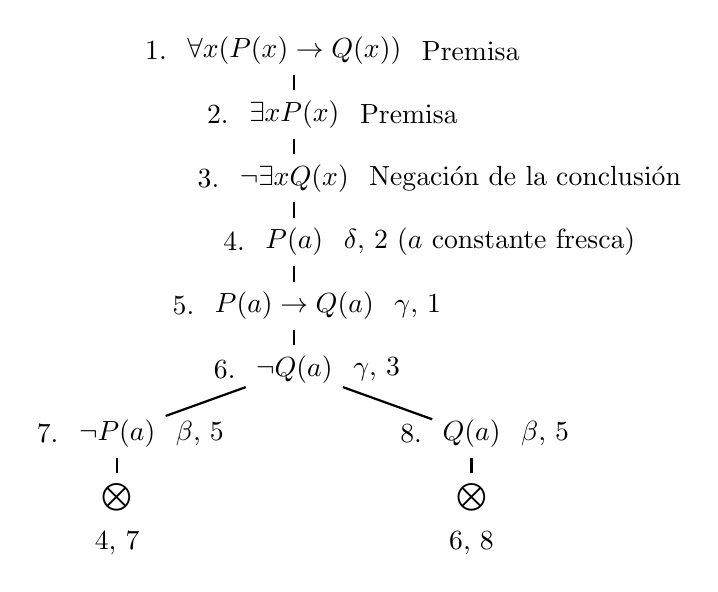
\begin{tikzpicture}[scale=0.9, -, thick, level/.style={sibling distance=5cm,level distance=.9cm}]
  \node[label=left:{1.},label=right:{Premisa}] (r1) {$\forall x (P(x) \to Q(x))$}
  child {
    node[label=left:{2.},label=right:{Premisa}] {$\exists x P(x)$}
    child {
      node[label=left:{3.},label=right:{Negación de la conclusión}] {$\neg \exists x Q(x)$}
      child {
        node[label=left:{4.},label=right:{$\delta$, 2 ($a$ constante fresca)}] {$P(a)$}
        child {
          node[label=left:{5.},label=right:{$\gamma$, 1}] {$P(a) \to Q(a)$}
          child {
            node[label=left:{6.},label=right:{$\gamma$, 3}] {$\neg Q(a)$}
            child {
              node[label=left:{7.},label=right:{$\beta$, 5}] {$\neg P(a)$}
              child { node[label=below:{4, 7}] {$\bigotimes$} }
            }
            child {
              node[label=left:{8.},label=right:{$\beta$, 5}] {$Q(a)$}
              child { node[label=below:{6, 8}] {$\bigotimes$} }
            }
          }
        }
      }
    }
  };
\end{tikzpicture}
\end{center}

\textbf{Comentario.} Seguimos el orden de prioridad de expansión:
\begin{enumerate}
    \item En el nodo 4 aplicamos primero la regla existencial $\delta$ sobre el nodo 2, generando la constante fresca $a$.
    \item Solo entonces instanciamos con esa constante $a$ las fórmulas $\gamma$ de los nodos 1 y 3 (nodos 5 y 6).
    \item Finalmente aplicamos la regla disyuntiva $\beta$ sobre el condicional (nodo 5). Ambas ramas chocan inmediatamente con literales previos: la rama izquierda ($\neg P(a)$) choca con el nodo 4 ($P(a)$), y la rama derecha ($Q(a)$) con el nodo 6 ($\neg Q(a)$).
    \item Todas las ramas están cerradas por contradicción ($\bigotimes$). Por consiguiente, el conjunto inicial es insatisfacible y la consecuencia semántica $\forall x (P(x) \to Q(x)), \exists x P(x) \models \exists x Q(x)$ queda demostrada.
\end{enumerate}
\end{ejemplo}

\begin{ejemplo}[Detección de invalidez y extracción sistemática de contramodelos]
Analicemos la inferencia (inválida) que «fusiona» dos existenciales en uno:
\[
\exists x P(x), \ \exists x Q(x) \ \stackrel{?}{\models} \ \exists x (P(x) \land Q(x))
\]
Colocamos las premisas y la negación de la conclusión en la raíz del árbol:

\begin{center}
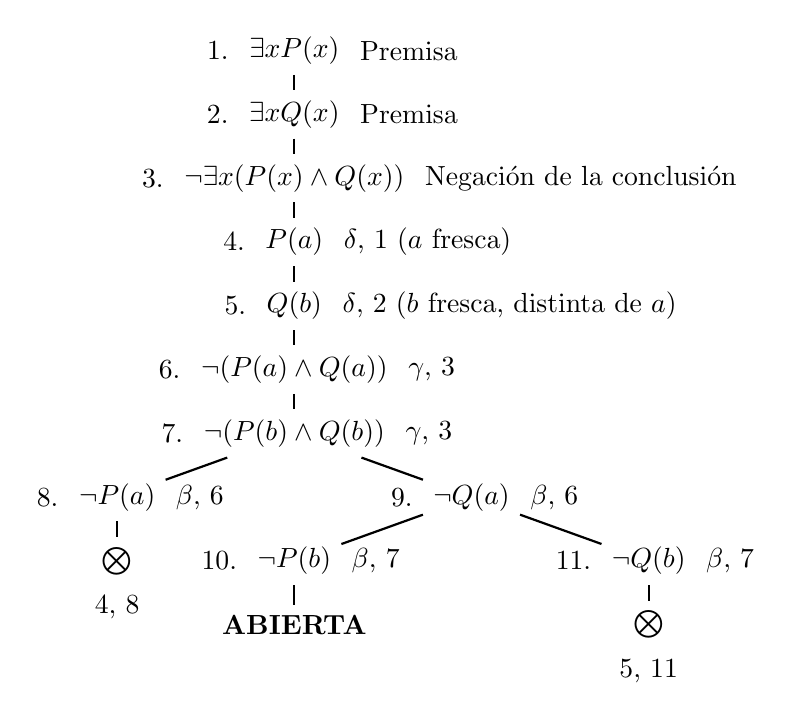
\begin{tikzpicture}[scale=0.9, -, thick, level/.style={sibling distance=5cm,level distance=.9cm}]
  \node[label=left:{1.},label=right:{Premisa}] (r1) {$\exists x P(x)$}
  child {
    node[label=left:{2.},label=right:{Premisa}] {$\exists x Q(x)$}
    child {
      node[label=left:{3.},label=right:{Negación de la conclusión}] {$\neg \exists x (P(x) \land Q(x))$}
      child {
        node[label=left:{4.},label=right:{$\delta$, 1 ($a$ fresca)}] {$P(a)$}
        child {
          node[label=left:{5.},label=right:{$\delta$, 2 ($b$ fresca, distinta de $a$)}] {$Q(b)$}
          child {
            node[label=left:{6.},label=right:{$\gamma$, 3}] {$\neg(P(a) \land Q(a))$}
            child {
              node[label=left:{7.},label=right:{$\gamma$, 3}] {$\neg(P(b) \land Q(b))$}
              child {
                node[label=left:{8.},label=right:{$\beta$, 6}] {$\neg P(a)$}
                child { node[label=below:{4, 8}] {$\bigotimes$} }
              }
              child {
                node[label=left:{9.},label=right:{$\beta$, 6}] {$\neg Q(a)$}
                child {
                  node[label=left:{10.},label=right:{$\beta$, 7}] {$\neg P(b)$}
                  child { node {\textbf{ABIERTA}} }
                }
                child {
                  node[label=left:{11.},label=right:{$\beta$, 7}] {$\neg Q(b)$}
                  child { node[label=below:{5, 11}] {$\bigotimes$} }
                }
              }
            }
          }
        }
      }
    }
  };
\end{tikzpicture}
\end{center}

\textbf{Comentario y extracción del contramodelo.} 
La rama abierta que desciende por los nodos 1--7, 9 y 10 no es un fallo del método, sino la construcción algorítmica de un contramodelo:
\begin{enumerate}
    \item \textbf{Dominio ($D$):} recogemos las constantes que ocurren en la rama abierta, $D = \{a, b\}$.
    \item \textbf{Literales de la rama:} $\Omega = \{P(a), Q(b), \neg Q(a), \neg P(b)\}$.
    \item \textbf{Extensiones de los predicados:} asignamos a cada predicado los elementos que aparecen afirmados:
    \[
    I(P) = \{a\}, \qquad I(Q) = \{b\}
    \]
    \item \textbf{Evaluación:} en esta estructura, el individuo $a$ cumple $P$ pero no $Q$, y el individuo $b$ cumple $Q$ pero no $P$. Las premisas son verdaderas ($\exists x P(x)$ por el individuo $a$, y $\exists x Q(x)$ por el individuo $b$), pero la conclusión es falsa (ningún individuo cumple simultáneamente $P$ y $Q$). El tableau ha construido un contramodelo formal que refuta la inferencia.
\end{enumerate}
\end{ejemplo}

\section{Los tableaux como cálculo\ampliacion}\label{sec:tableaux-calculo}

El nombre de «tableaux semánticos» tiene una razón histórica. Gentzen
había introducido en 1934 el cálculo de secuentes con una motivación
sintáctica: analizar la estructura de las pruebas. Beth y Hintikka,
que propusieron el método de los tableaux de forma independiente en
1955, partían en cambio de una preocupación semántica. Beth lo
concebía como un intento de construir un contraejemplo,
que se encontrará si y solo si el argumento no es válido. Esa búsqueda
debe llevarse a cabo de forma sistemática, y eso es lo que hace un tableau semántico (Beth, 1955). Su tabla tenía dos columnas, una para las fórmulas que deben ser verdaderas y otra para las que deben ser falsas. Hintikka entendía del mismo modo las pruebas de verdad lógica, como pruebas de que es imposible un contraejemplo, y caracterizó los conjuntos que hoy llevan su nombre (él los llamó \emph{conjuntos modelo}), que describen parcialmente un modelo (Hintikka, 1955). Más tarde, Smullyan (1968) habló de \emph{tableaux analíticos}, para destacar que en ellos solo intervienen subfórmulas de las fórmulas de partida. Fitting (1999) cuenta esta historia con detalle.

Esa motivación explica que a menudo se vean como un procedimiento semántico. Pero son, como la deducción natural, un cálculo de demostración en sentido estricto. Sus reglas son sintácticas: indican qué fórmulas se añaden a una rama según la forma de las que ya contiene ($\alpha$, $\beta$, $\gamma$, $\delta$), y una rama se cierra cuando contiene una fórmula y su negación. Para aplicarlas, y para comprobar que un tableau está bien construido, no hace falta interpretar ningún símbolo, igual que ocurre con una derivación de Fitch. Por eso el cálculo tiene su propia relación de derivabilidad: escribimos $\Gamma \vdash_T A$ cuando hay un tableau cerrado para $\Gamma \cup \{\neg A\}$.

La semántica interviene en dos lugares, pero fuera del cálculo. Primero, en la motivación: cada regla está pensada para reflejar las condiciones de verdad de una conectiva o de un cuantificador, como ocurre con las reglas de introducción y eliminación de la deducción natural. Segundo, en la lectura de los resultados: entendemos que un tableau cerrado muestra que no hay modelo y que una rama abierta y completa describe uno. Que esas lecturas sean adecuadas no es evidente; son los teoremas de corrección y completud del cálculo de tableaux (sección siguiente), que relacionan $\vdash_T$ con $\models$ como los temas~\ref{cap:meta-prop} y~\ref{cap:sem-lpo} relacionaban la derivabilidad en deducción natural con la consecuencia lógica. 

Lo que distingue a los tableaux de la deducción natural no es, por
tanto, que uno sea semántico y el otro sintáctico, sino el modo de
construir las pruebas. La deducción natural es sintética: construye la
conclusión a partir de las premisas. Los tableaux son analíticos:
descomponen las fórmulas de partida y solo añaden fórmulas obtenidas
de ellas (sus componentes, a veces negados, o sus instancias). Un
tableau no construye la conclusión; lo que puede construir, cuando una
rama queda abierta, es un modelo. En esto sí se distinguen los
tableaux de la mayoría de los demás cálculos: cuando en un sistema
axiomático o en deducción natural no se encuentra una prueba, el
intento fallido no proporciona un contramodelo, mientras que una rama
abierta y completa describe uno. Como ha señalado P. de Rouilhan
(1998-1999), los tableaux son un método sintáctico, y su aspecto
semántico es un subproducto cuando fracasa en un intento de prueba. 

\section{Metalógica de tableaux: corrección y completud\ampliacion}

Al igual que la deducción natural, el cálculo de tableaux es un sistema deductivo adecuado:

\begin{theorem}[Corrección del cálculo de tableaux]
Si existe un tableau cerrado para $\Gamma \cup \{\neg A\}$ (es decir, si $\Gamma \vdash_T A$), entonces $\Gamma \models A$.  
(En particular, si hay un tableau cerrado para $\Gamma$, $\Gamma$ es insatisfacible).
\end{theorem}

\begin{proof}[Idea de la demostración]
La prueba descansa en la noción de \textbf{satisfacibilidad de una rama}: decimos que una rama $\mathcal{B}$ es satisfacible si existe al menos una estructura $\mathcal{M}$ en la que todas las fórmulas que pertenecen a $\mathcal{B}$ son verdaderas.
\begin{enumerate}
    \item Se demuestra inductivamente que todas las reglas de expansión preservan la satisfacibilidad:
    \begin{itemize}
        \item Si una rama satisfacible se expande mediante una regla $\alpha$, la única rama resultante sigue siendo satisfacible (pues $\alpha \equiv \alpha_1 \land \alpha_2$).
        \item Si se expande mediante una regla $\beta$, al menos una de las dos ramas hijas resultantes es satisfacible (pues $\beta \equiv \beta_1 \lor \beta_2$).
        \item Si se expande mediante una regla $\delta$, al introducir una constante fresca $a$, siempre podemos extender la interpretación asignando a $a$ el testigo que garantiza la verdad del existencial, manteniendo la rama satisfacible.
        \item La regla $\gamma$ preserva la satisfacibilidad trivialmente, pues si $\forall x A(x)$ es verdadera, cualquier instancia $A(c)$ lo es. (Si $\gamma$ introduce una constante nueva porque la rama no tenía ninguna, se le asigna cualquier elemento del dominio; al ser nueva, no altera el valor de las demás fórmulas).
        \item La regla $\sigma$ también la preserva trivialmente, pues $\neg\neg A \equiv A$.
    \end{itemize}
    \item Ahora bien, si un tableau es cerrado, todas sus ramas contienen una fórmula y su negación, y ninguna rama cerrada es satisfacible.
    \item Por tanto, si el conjunto inicial $\Gamma \cup \{\neg A\}$ fuera satisfacible, el árbol debería contener al menos una rama abierta satisfacible. Al no existir ninguna, se concluye que $\Gamma \cup \{\neg A\}$ es insatisfacible, de donde $\Gamma \models A$. \qedhere
\end{enumerate}
\end{proof}

\begin{theorem}[Completud del cálculo de tableaux]
Sea $\Gamma$ finito. Si $\Gamma \models A$, entonces cualquier tableau
para $\Gamma \cup \{\neg A\}$ construido de forma sistemática (sin que
ninguna fórmula quede sin expandir indefinidamente) se termina
cerrando. En particular, $\Gamma \vdash_T A$.  
\end{theorem}

\begin{proof}[Idea de la demostración (vía conjuntos de Hintikka)]
Razonamos por el contrarrecíproco. Si el árbol sistemático completo para $\Gamma \cup \{\neg A\}$ no se cierra, contiene al menos una rama abierta $\mathcal{B}$, quizá infinita. 
\begin{enumerate}
    \item Por la sistematicidad de la aplicación de reglas, el conjunto de fórmulas de dicha rama abierta $\mathcal{B}$ forma un \textbf{conjunto de Hintikka}:
    \begin{itemize}
        \item No contiene ninguna contradicción atómica ($P \in \mathcal{B} \implies \neg P \notin \mathcal{B}$).
        \item Si $\neg\neg A \in \mathcal{B}$, entonces $A \in \mathcal{B}$.
        \item Si $\alpha \in \mathcal{B}$, entonces $\alpha_1 \in \mathcal{B}$ y $\alpha_2 \in \mathcal{B}$.
        \item Si $\beta \in \mathcal{B}$, entonces $\beta_1 \in \mathcal{B}$ o $\beta_2 \in \mathcal{B}$.
        \item Si $\delta \in \mathcal{B}$, existe una constante $a$ tal que $\delta(a) \in \mathcal{B}$.
        \item Si $\gamma \in \mathcal{B}$, para toda constante $c$ que aparezca en la rama, $\gamma(c) \in \mathcal{B}$ (y en la rama aparece al menos una constante).
    \end{itemize}
    \item Por el \textbf{lema de Hintikka}, todo conjunto de Hintikka es satisfacible: basta construir la estructura canónica sobre las constantes de la rama (exactamente como en el teorema de extracción del modelo).
    \item Dicha estructura satisface todas las fórmulas de la rama $\mathcal{B}$, incluyendo las premisas $\Gamma$ y la negación $\neg A$.
    \item La existencia de esta estructura demuestra que $\Gamma \not\models A$. Por tanto, si $\Gamma \models A$, el tableau sistemático se cierra. \qedhere
\end{enumerate}
\end{proof}

\section{Ramas infinitas y la semidecidibilidad de primer orden}\label{sec:ramas-infinitas}

En lógica proposicional, todo tableau es finito: cada paso descompone
fórmulas en subfórmulas más pequeñas o en sus negaciones (el
bicondicional, a través de una conjunción de ellas) y nunca se repite la aplicación
de una regla sobre una misma fórmula. Por ello, el proceso concluye
siempre en un número finito de pasos (decidibilidad).

En lógica de primer orden la finitud del tableau no está
garantizada. Consideremos como ejemplo el conjunto de premisas:  
\[
\Gamma = \{\forall x \exists y R(x, y), \ \forall x \neg R(x, x)\}
\]
\begin{enumerate}
    \item Empezamos con una constante $c_1$. Por $\forall x \exists y R(x, y)$, obtenemos $\exists y R(c_1, y)$.
    \item Por la regla $\delta$, el existencial exige crear una constante fresca $c_2$, obteniendo $R(c_1, c_2)$.
    \item Pero ahora $c_2$ debe ser procesada por el universal $\forall x \exists y R(x, y)$, produciendo $\exists y R(c_2, y)$.
    \item Al aplicar $\delta$, debemos crear otra constante fresca, $c_3$, obteniendo $R(c_2, c_3)$, y así indefinidamente.
\end{enumerate}

El tableau genera una rama abierta infinita:
\[
c_1 \xrightarrow{R} c_2 \xrightarrow{R} c_3 \xrightarrow{R} c_4 \xrightarrow{R} \dots
\]

\paragraph{Ramas infinitas y modelos finitos: una limitación algorítmica.}
Conviene advertir que la aparición de esta rama infinita no significa
que $\Gamma$ solo pueda satisfacerse en dominios infinitos. De hecho,
el conjunto anterior posee un modelo finito con solo dos elementos:
\[
D = \{1, 2\}, \quad I(R) = \{(1, 2), \ (2, 1)\}
\]
(donde el 1 se relaciona con el 2, el 2 con el 1, y ningún elemento se relaciona consigo mismo). Si no tuviéramos la condición de irreflexividad $\forall x \neg R(x, x)$, la fórmula $\forall x \exists y R(x, y)$ se satisfaría trivialmente en un dominio de un solo elemento con $I(R) = \{(1, 1)\}$.

¿Por qué entonces el tableau no se detiene? La causa está en la regla $\delta$ estándar, que obliga a introducir una constante \emph{fresca} para cada fórmula existencial, sin comprobar si alguna de las constantes ya disponibles en la rama (por ejemplo, $c_1$ como testigo de $\exists y R(c_2, y)$) permitiría satisfacer la fórmula sin agrandar el dominio.

Existen modificaciones del método de árboles diseñadas para paliar este problema (véase Boolos, 1984). En dichas variantes, ante una fórmula existencial en una rama donde ya existen constantes $\{c_1, \dots, c_k\}$, el árbol se bifurca explorando ramas para cada una de las constantes previas y una rama adicional con una constante nueva. Esa ramificación permite al cálculo encontrar modelos finitos (siempre que existan) y detenerse con éxito en ejemplos como el anterior.

\practica{En \apptableaux{} se ven las dos situaciones con este ejemplo: con la regla $\delta$ estándar la rama queda incompleta al llegar al límite de constantes, y con la opción «Regla $\delta$ de Boolos» aparece el modelo finito de dos elementos.}

\paragraph{La barrera de la indecidibilidad (Church-Turing).}
No obstante, ninguna variante algorítmica puede evitar las ramas infinitas en todos los casos: si pudiera, tendríamos un procedimiento de decisión para la lógica de primer orden, lo que contradice el teorema de Church y Turing. Un ejemplo concreto lo dan los conjuntos de fórmulas satisfacibles que solo tienen modelos infinitos: por ejemplo, si al conjunto $\Gamma$ le añadimos la propiedad transitiva $\forall x \forall y \forall z (R(x, y) \land R(y, z) \to R(x, z))$, se define un orden estricto serial, que carece de modelos finitos. En tal caso, ningún tableau puede terminar con una rama abierta y finita, porque de ella se extraería un modelo finito: la rama abierta ha de ser infinita.

Este comportamiento refleja las propiedades metalógicas de la lógica de primer orden:
\begin{itemize}
    \item \textbf{Semidecidibilidad de LPO (consecuencia de la completud).} Si un argumento con un número finito de premisas es válido ($\Gamma \models A$), el tableau construido de modo sistemático se cerrará siempre en un número finito de pasos.
    \item \textbf{Indecidibilidad de LPO (Church-Turing).} Si el argumento no es válido, el algoritmo de tableaux puede permanecer ejecutándose indefinidamente en una rama infinita sin que exista ningún procedimiento mecánico general que decida si el árbol terminará cerrándose o no.
\end{itemize}
Más que un defecto del método, las ramas infinitas hacen visible en el propio árbol un límite de lo computable.

\section*{Referencias bibliográficas}

\begin{enumerate}
    \item \textbf{Beth, E. W.} (1955). «Semantic entailment and formal derivability». \emph{Mededelingen der Koninklijke Nederlandse Akademie van Wetenschappen, Afd. Letterkunde}, nueva serie, vol. 18, n.º 13, pp. 309--342. [Introducción original de los tableaux semánticos].
    \item \textbf{Boolos, G.} (1984). «Trees and finite satisfiability: proof of a conjecture of Burgess». \emph{Notre Dame Journal of Formal Logic}, vol. 25, n.º 3, pp. 193--197. [Variante de la regla existencial que encuentra modelos finitos cuando existen].
    \item \textbf{D'Agostino, M.} (1992). «Are tableaux an improvement on truth-tables? Cut-free proofs and bivalence». \emph{Journal of Logic, Language and Information}, vol. 1, n.º 3, pp. 235--252.
    \item \textbf{Fitting, M.} (1996). \emph{First-Order Logic and Automated Theorem Proving} (2.ª ed.). Springer. [Exposición moderna orientada a demostración automática y conjuntos de Hintikka].
    \item \textbf{Fitting, M.} (1999). «Introduction». En D'Agostino, M., Gabbay, D. M., Hähnle, R., \& Posegga, J. (eds.), \emph{Handbook of Tableau Methods}. Kluwer Academic Publishers. [Historia de los métodos de tableaux, de Gentzen y Beth a la demostración automática].
    \item \textbf{Hintikka, J.} (1955). «Form and content in quantification theory». \emph{Acta Philosophica Fennica}, vol. 8, pp. 7--55. [Conjuntos modelo, hoy llamados conjuntos de Hintikka].
    \item \textbf{Robinson, J. A.} (1965). «A machine-oriented logic based on the resolution principle». \emph{Journal of the ACM}, vol. 12, n.º 1, pp. 23--41. [El método de resolución, base de muchos demostradores automáticos y de la programación lógica].
    \item \textbf{Rouilhan, P. de} (1998-1999). «Les tableaux de Beth: syntaxe ou sémantique?». \emph{Philosophia Scientiae}, vol. 3, n.º 4, pp. 303--322. [Sobre el carácter sintáctico de los tableaux].
    \item \textbf{Smullyan, R. M.} (1968). \emph{First-Order Logic}. Springer-Verlag. [La formulación uniforme de los tableaux].
\end{enumerate}

%%% Local Variables:
%%% mode: latex
%%% TeX-master: "ApuntesLogica"
%%% End:
